\section{Техническое задание}
\subsection{Основание для разработки}

Полное наименование системы: «Программная реализация системы управления проектами». Основанием для разработки программы является приказ ректора ЮЗГУ от «17» апреля 2025 г. № 1828-с приказа «О направлении (допуске) на практику». %«Об утверждении тем выпускных квалификационных работ».

\subsection{Цель и назначение разработки}

Система управления проектами предназначена для эффективной организации, отслеживания и координации рабочих процессов команд, использующих гибкие методологии Agile и, в частности, Kanban-подход, с целью повышения прозрачности, предсказуемости и продуктивности выполнения проектов.
Пользователи (включая менеджеров проектов, владельцев продуктов, разработчиков и других членов команды) должны иметь возможность визуализировать этапы работы с помощью настраиваемых Kanban-досок, управлять потоком задач от создания до завершения, отслеживать прогресс в реальном времени и анализировать эффективность процессов для непрерывного улучшения. Система должна предоставлять интуитивно понятный интерфейс для совместной работы и обеспечивать легкий доступ ко всей необходимой проектной информации.
Задачами данной разработки являются:
\begin{enumerate}
	\item Создание основной архитектуры и серверной логики для управления проектами, Kanban-досками, задачами (карточками), пользователями и их ролями.
	\item Разработка веб-интерфейса пользователя с интерактивной Kanban-доской, поддерживающей создание и настройку колонок, перемещение задач, установку WIP-лимитов и визуализацию статусов задач.
	\item Реализация функционала управления задачами, включая их создание, редактирование, назначение ответственных, установку приоритетов, сроков выполнения, добавление описаний, чек-листов, меток (тегов) и прикрепление файлов.
	\item Интеграция инструментов для поддержки Agile-практик, таких как управление бэклогом продукта, планирование итераций, а также базовые метрики для отслеживания производительности.
	\item Разработка системы уведомлений и средств для совместной работы, включая комментирование задач, упоминания пользователей и отслеживание истории изменений.
	\item Обеспечение базовых функций администрирования системы, включая управление пользователями, настройку прав доступа и управление проектными пространствами.
\end{enumerate}


\subsection{Актуальность темы разработки}
В условиях современной цифровой экономики, характеризующейся высокой скоростью изменений, глобализацией рынков и постоянно растущей конкуренцией, способность компаний быстро и эффективно реализовывать проекты становится критически важным фактором успеха. Особенно остро это проявляется в сфере информационных технологий и разработки программного обеспечения, где жизненные циклы продуктов сокращаются, а требования заказчиков и пользователей эволюционируют с беспрецедентной скоростью. По состоянию на 2025 год, организации всех размеров активно ищут инструменты и подходы, позволяющие им не только управлять проектами, но и гибко адаптироваться к непредвиденным обстоятельствам, сохраняя при этом фокус на создании ценности.

Актуальность разработки такой системы обусловлена, прежде всего, повышенным спросом на гибкость и адаптивность, поскольку современные проекты требуют от команд способности быстро перестраиваться, изменять приоритеты и инкорпорировать новые требования без значительных потерь времени и ресурсов, чему идеально отвечает комбинированный подход Agile и Kanban. Эта потребность в адаптивных инструментах становится особенно острой в условиях роста популярности удаленных и гибридных моделей работы, что порождает необходимость в эффективных цифровых решениях, способных обеспечить прозрачность, синхронизацию и эффективную коллаборацию всех участников проекта независимо от их местоположения; здесь программно реализованная Kanban-доска выступает как единый источник правды для команды. Кроме того, интегрированная система напрямую способствует стремлению к повышению производительности и сокращению потерь, позволяя не только визуализировать задачи, но и отслеживать метрики производительности, такие как время цикла и пропускная способность, а также применять WIP-лимиты для предотвращения перегрузок и фокусировки на завершении начатой работы, что ведет к повышению общей эффективности. 

Несмотря на наличие на рынке множества систем управления проектами, сохраняется выраженный запрос на инструменты, которые можно легко адаптировать под специфические процессы конкретной команды или организации, и которые обладают интуитивно понятным интерфейсом и низким порогом вхождения для пользователей. В конечном итоге, предлагаемая программная система поддерживает культуру непрерывного улучшения, поощряемую как Agile, так и Kanban, предоставляя ценные данные для проведения ретроспектив и анализа эффективности потока работ.
\subsection{Этапы разработки}

Для реализации программной системы предполагается выполнение следующих этапов:
\begin{enumerate}
	\item Анализ предметной области и определение ключевых требований к функционалу Kanban-доски и интеграции Agile-методик.
	\item Проектирование архитектуры приложения.
	\item Разработка структуры базы данных для хранения информации об основных сущностях системы, их состояниях и прочей технической информации.
	\item Реализация серверной логики и API для управления основными сущностями системы.
	\item Создание пользовательского интерфейса для удобного пользования приложением.
	\item Проведение функционального тестирования для выявления критичных несоответствий.
\end{enumerate}

\subsection{Требования к программной системе}

\subsubsection{Требования к данным}
Входными данными для системы являются:
\begin{itemize}
	\item учетные данные пользователя;
	\item параметры задач, проектов, досок;
	\item комментарии к задачам.
\end{itemize}
Выходными данными для системы являются:
\begin{itemize}
	\item полная и детализированная информация о пользователях, задачах, проектах, досках;
	\item системные уведомления и информационные сообщения.
\end{itemize}

\subsubsection{Функциональные требования}
В разрабатываемой системе управления проектами должно быть предусмотрено наличие трех основных ролей пользователей с различными наборами прав и функциональных возможностей в рамках каждого проекта: «Участник проекта», «Владелец проекта» и «Администратор».

Пользователю  с ролью «Участник проекта» должны  быть доступны следующие функции:
\begin{itemize}
	\item регистрация и аутентификация;
	\item просмотр и изменение персональной информации;
	\item удаление профиля;
	\item просмотр проектов, в которых он состоит, и существующих в них досок;
	\item просмотр, создание, редактирование, перемещение всех задач;
	\item удаление собственных задач.
\end{itemize}

Пользователю  с ролью «Владелец проекта» должны  быть доступны следующие функции:
\begin{itemize}
	\item регистрация и аутентификация;
	\item просмотр и изменение персональной информации;
	\item удаление профиля;
	\item просмотр, создание, редактирование, удаление собственных проектов и досок;
	\item просмотр, создание, редактирование, перемещение, удаление любых задач в собственных проектах независимо от автора;
	\item управление участниками собственных проектов.
\end{itemize}

Пользователю  с ролью «Администратор» должны  быть доступны следующие функции:
\begin{itemize}
	\item регистрация и аутентификация;
	\item просмотр и изменение персональной информации;
	\item удаление профиля;
	\item просмотр, создание, редактирование, удаление всех существующих проектов, досок и задач (а также их перемещение);
	\item управление участниками всех проектов.
\end{itemize}

На рисунке ~\ref{use_case_diagram:image} представлена диаграмма прецедентов.

\begin{figure}[H]
	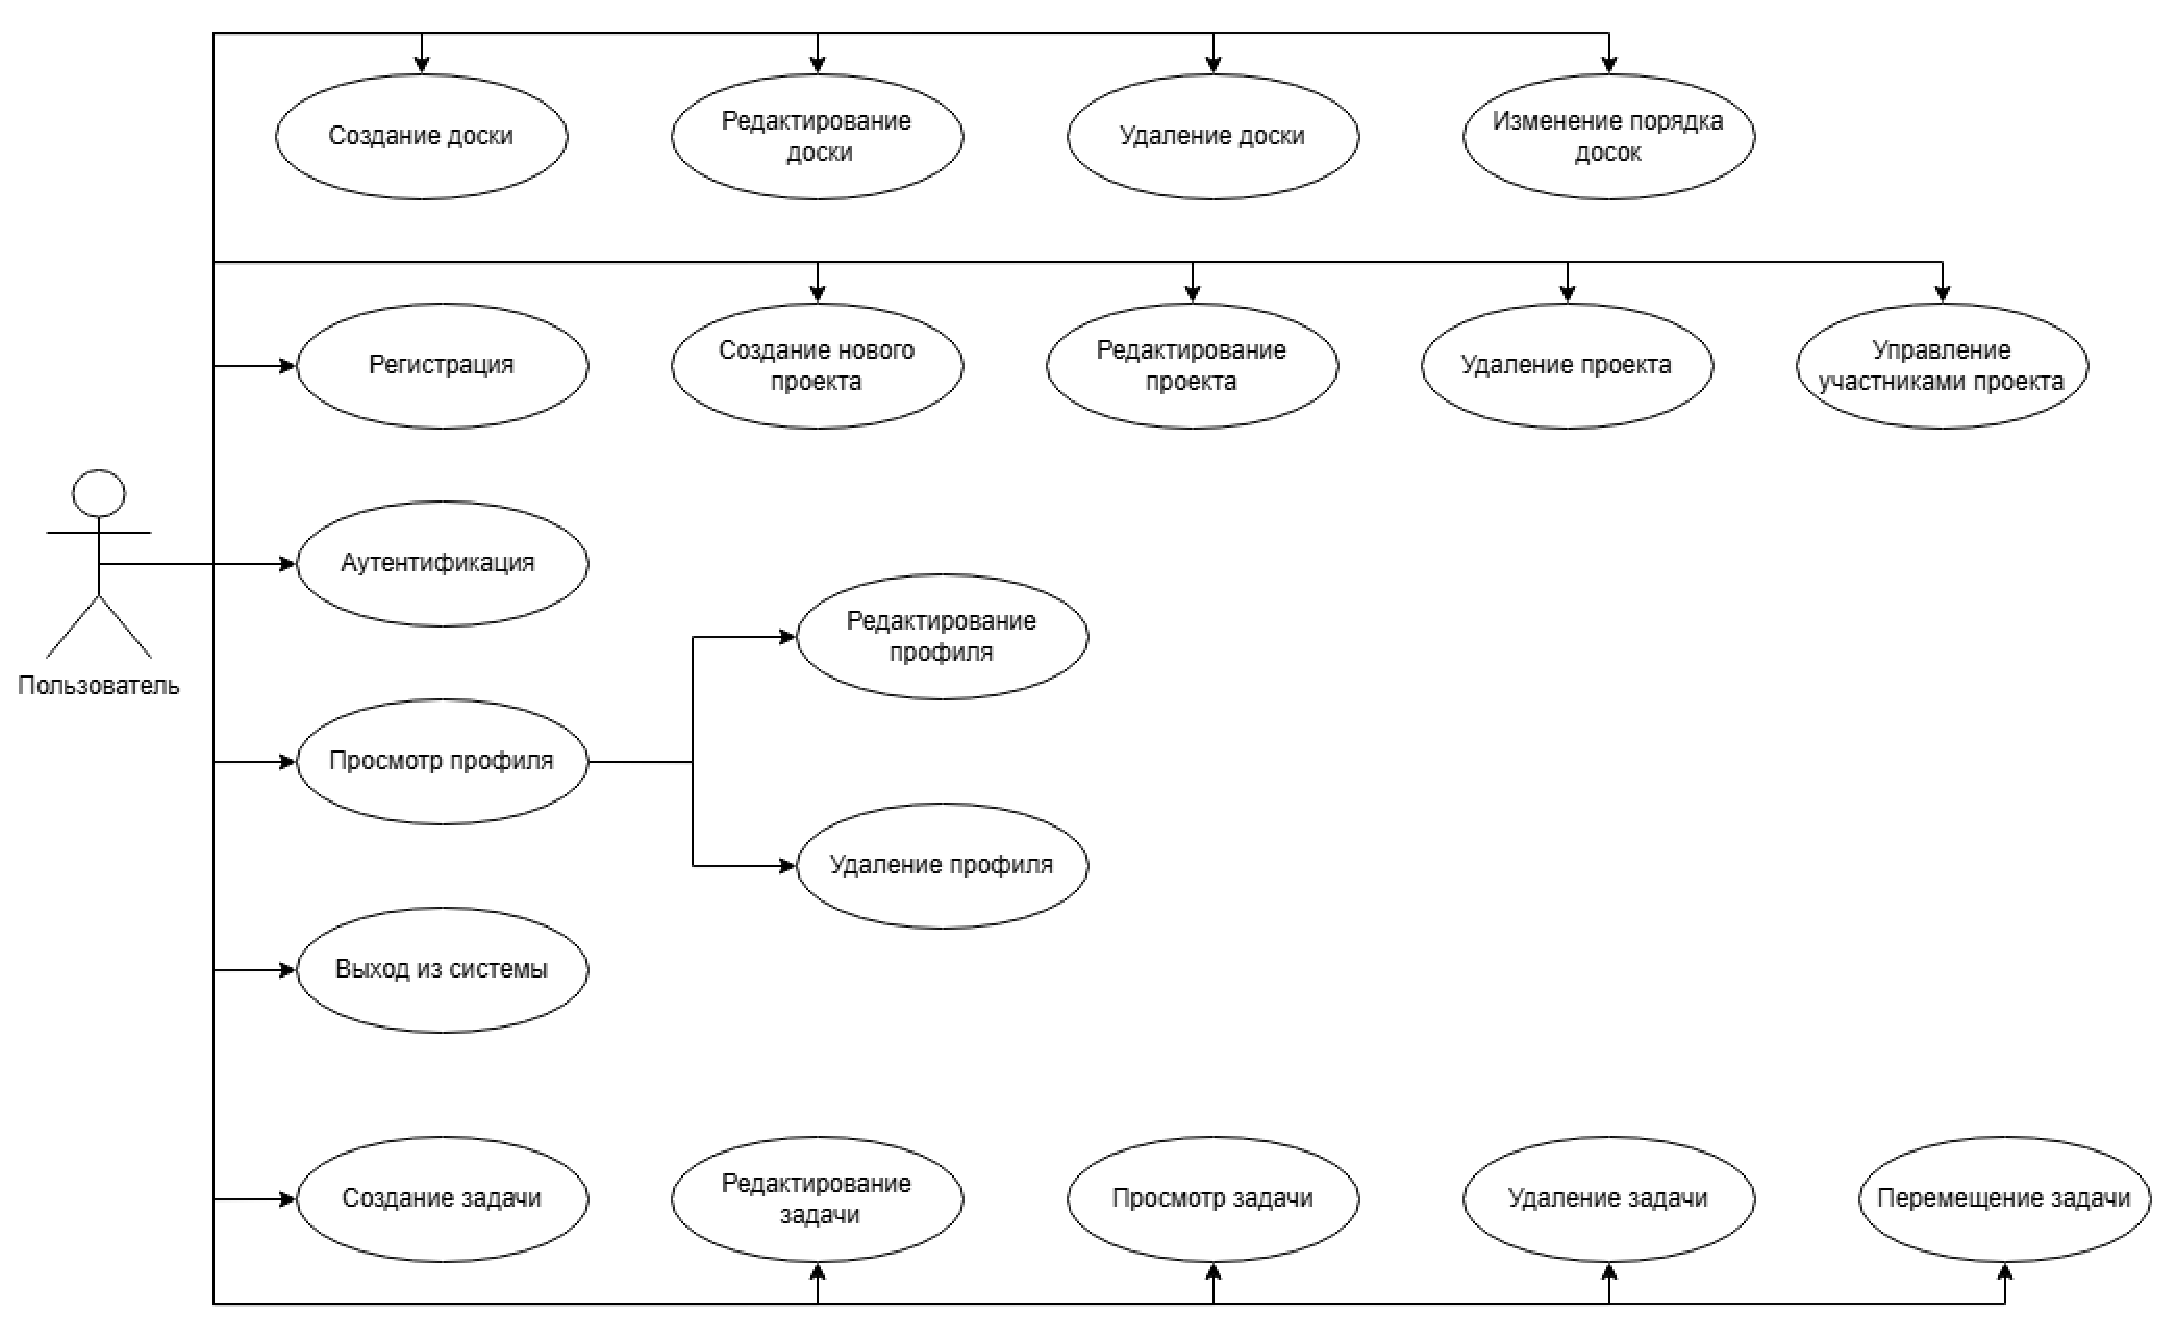
\includegraphics[width=1\linewidth]{use_case_diagram}
	\caption{Диаграмма прецедентов}
	\label{use_case_diagram:image}
\end{figure}


\subsubsection{Сценарий прецедента «Регистрация»}
Основной успешный сценарий:
\begin{enumerate}
	\item Пользователь переходит на страницу аутентификации web-приложения.
	\item Пользователь нажимает на ссылку/кнопку «Создать».
	\item Пользователь вводит свое имя в поле «Имя».
	\item Пользователь вводит свою фамилию в поле «Фамилия».
	\item Пользователь вводит свой адрес электронной почты в поле «Адрес электронной почты».
	\item Пользователь вводит свой пароль в поле «Пароль», соблюдая указанные критерии.
	\item Пользователь подтверждает свой пароль в поле «Подтвердите пароль».
	\item Пользователь нажимает кнопку «Создать аккаунт».
	\item Система проверяет корректность введенных данных и уникальность email.
	\item Система регистрирует нового пользователя.
	\item Система автоматически аутентифицирует пользователя, сохраняет токен и перенаправляет его на основной интерфейс приложения (доску Kanban).
\end{enumerate}

\subsubsection{Сценарий прецедента «Аутентификация»}
Основной успешный сценарий:
\begin{enumerate}
	\item Пользователь переходит на страницу аутентификации web-приложения.
	\item Пользователь вводит свой адрес электронной почты в поле «Адрес электронной почты».
	\item Пользователь вводит свой пароль в поле «Пароль».
	\item Пользователь нажимает кнопку «Войти».
	\item Система проверяет корректность введенных учетных данных.
	\item Система аутентифицирует пользователя, сохраняет токен и перенаправляет его на основной интерфейс приложения (доску Kanban).
\end{enumerate}

\subsubsection{Сценарий прецедента «Выход из системы»}
Основной успешный сценарий:
\begin{enumerate}
	\item Аутентифицированный пользователь нажимает на иконку «Выйти» на панели настроек.
	\item Система отображает модальное окно с запросом подтверждения выхода.
	\item Пользователь нажимает кнопку «Выйти» в модальном окне.
	\item Система завершает сеанс пользователя (удаляет токен).
	\item Система перенаправляет пользователя на страницу аутентификации.
\end{enumerate}

\subsubsection{Сценарий прецедента «Просмотр профиля»}
Основной успешный сценарий:
\begin{enumerate}
	\item Аутентифицированный пользователь нажимает на иконку «Профиль пользователя» на панели настроек.
	\item Система отображает страницу профиля пользователя с его данными (ФИО, email, дата регистрации, аватар).
\end{enumerate}

\subsubsection{Сценарий прецедента «Редактирование профиля»}
Основной успешный сценарий:
\begin{enumerate}
	\item Пользователь находится на странице своего профиля.
	\item Пользователь нажимает кнопку «Редактировать профиль».
	\item Система отображает модальное окно редактирования профиля с текущими данными.
	\item Пользователь изменяет необходимые поля (имя, фамилия, отчество, URL аватара).
	\item Пользователь нажимает кнопку «Сохранить изменения».
	\item Система проверяет корректность введенных данных.
	\item Система обновляет данные профиля пользователя в базе данных.
	\item Система обновляет данные профиля в интерфейсе и закрывает модальное окно.
\end{enumerate}

\subsubsection{Сценарий прецедента «Удаление профиля»}
Основной успешный сценарий:
\begin{enumerate}
	\item Пользователь находится на странице своего профиля.
	\item Пользователь нажимает кнопку «Удалить профиль».
	\item Система отображает модальное окно с запросом подтверждения удаления профиля.
	\item Пользователь нажимает кнопку «Да, удалить мой профиль».
	\item Система удаляет профиль пользователя из базы данных.
	\item Система завершает сеанс пользователя и перенаправляет на страницу аутентификации.
\end{enumerate}

\subsection*{Управление Проектами}

\subsubsection{Сценарий прецедента «Создание нового проекта»}
Основной успешный сценарий:
\begin{enumerate}
	\item Аутентифицированный пользователь нажимает на иконку «Добавить новый проект» на панели настроек.
	\item Система отображает модальное окно для добавления проекта.
	\item Пользователь вводит название проекта в поле «Название проекта».
	\item Пользователь опционально вводит описание проекта в поле «Описание».
	\item Пользователь нажимает кнопку «Создать проект».
	\item Система создает новый проект в базе данных, назначая текущего пользователя владельцем.
	\item Система добавляет владельца в участники проекта.
	\item Система обновляет список проектов в интерфейсе, новый проект становится текущим (если это первый проект или по логике приложения).
	\item Модальное окно закрывается.
\end{enumerate}

\subsubsection{Сценарий прецедента «Редактирование проекта»}
Условия: Пользователь является владельцем проекта или администратором.
Основной успешный сценарий:
\begin{enumerate}
	\item Пользователь (владелец/админ) нажимает на иконку «Редактировать текущий проект» на панели настроек (кнопка активна, если проект выбран).
	\item Система отображает модальное окно редактирования текущего проекта с его данными.
	\item Пользователь изменяет название и/или описание проекта.
	\item Пользователь нажимает кнопку «Сохранить изменения».
	\item Система обновляет данные проекта в базе данных.
	\item Система обновляет название/описание проекта в интерфейсе. Модальное окно может закрыться или показать сообщение об успехе.
\end{enumerate}

\subsubsection{Сценарий прецедента «Удаление проекта»}
Условия: Пользователь является владельцем проекта или администратором.
Основной успешный сценарий:
\begin{enumerate}
	\item Пользователь (владелец/админ) открывает модальное окно редактирования проекта.
	\item Пользователь нажимает кнопку «Удалить проект».
	\item Система отображает модальное окно подтверждения удаления проекта.
	\item Пользователь нажимает кнопку «Да, удалить проект».
	\item Система удаляет проект, все связанные с ним доски и задачи из базы данных.
	\item Система обновляет список проектов в интерфейсе. Если удален текущий проект, выбирается другой или отображается состояние "нет проектов".
	\item Модальные окна закрываются.
\end{enumerate}

\subsubsection{Сценарий прецедента «Управление участниками проекта»}
Условия: Пользователь является владельцем проекта или администратором.
Основной успешный сценарий (Просмотр):
\begin{enumerate}
	\item Пользователь (владелец/админ) нажимает на иконку «Управление участниками проекта» на панели настроек (кнопка активна, если проект выбран).
	\item Система отображает модальное окно со списком текущих участников проекта.
\end{enumerate}
Основной успешный сценарий (Добавление участника):
\begin{enumerate}
	\item В модальном окне управления участниками пользователь вводит email существующего пользователя системы в поле «Введите email пользователя для добавления».
	\item Пользователь нажимает кнопку «Добавить».
	\item Система проверяет, существует ли пользователь с таким email и не является ли он уже участником.
	\item Система добавляет пользователя в участники проекта.
	\item Список участников в модальном окне обновляется.
\end{enumerate}
Основной успешный сценарий (Удаление участника):
\begin{enumerate}
	\item В модальном окне управления участниками пользователь нажимает иконку удаления напротив участника (не владельца).
	\item Система удаляет пользователя из участников проекта.
	\item Список участников в модальном окне обновляется.
\end{enumerate}

\subsubsection{Сценарий прецедента «Создание доски»}
Условия: Пользователь является владельцем текущего проекта или администратором. Проект выбран.
Основной успешный сценарий:
\begin{enumerate}
	\item Пользователь (владелец/админ) нажимает на иконку «Добавить новую доску» на панели настроек.
	\item Система отображает модальное окно для добавления доски.
	\item Пользователь вводит название доски в поле «Заголовок доски».
	\item Пользователь опционально вводит описание доски.
	\item Пользователь нажимает кнопку «Добавить доску».
	\item Система создает новую доску в текущем проекте.
	\item Система обновляет интерфейс, отображая новую доску в конце списка досок текущего проекта.
	\item Модальное окно закрывается.
\end{enumerate}

\subsubsection{Сценарий прецедента «Редактирование доски»}
Условия: Пользователь является владельцем проекта, к которому принадлежит доска, или администратором.
Основной успешный сценарий:
\begin{enumerate}
	\item Пользователь нажимает на иконку редактирования на заголовке доски.
	\item Система отображает модальное окно редактирования доски с ее текущими данными.
	\item Пользователь изменяет название и/или описание доски.
	\item Пользователь нажимает кнопку «Сохранить».
	\item Система обновляет данные доски в базе данных.
	\item Система обновляет отображение доски в интерфейсе. Модальное окно закрывается.
\end{enumerate}

\subsubsection{Сценарий прецедента «Удаление доски»}
Условия: Пользователь является владельцем проекта, к которому принадлежит доска, или администратором.
Основной успешный сценарий:
\begin{enumerate}
	\item Пользователь открывает модальное окно редактирования доски.
	\item Пользователь нажимает кнопку «Удалить доску».
	\item Система (опционально) запрашивает подтверждение.
	\item Система удаляет доску и все связанные с ней задачи.
	\item Система обновляет интерфейс, убирая доску. Модальное окно закрывается.
\end{enumerate}

\subsubsection{Сценарий прецедента «Изменение порядка досок»}
Основной успешный сценарий:
\begin{enumerate}
	\item Аутентифицированный пользователь наводит курсор на заголовок доски.
	\item Пользователь зажимает левую кнопку мыши на заголовке доски и перетаскивает доску на новую позицию среди других досок текущего проекта.
	\item Пользователь отпускает кнопку мыши.
	\item Система визуально обновляет порядок досок на экране.
	\item Система сохраняет новый порядок отображения досок для текущего проекта в базе данных.
\end{enumerate}

\subsubsection{Сценарий прецедента «Создание  задачи»}
Условия: Пользователь аутентифицирован, проект выбран, и пользователь является участником проекта (или владельцем/администратором).
Основной успешный сценарий:
\begin{enumerate}
	\item Пользователь нажимает на иконку «Добавить новую задачу» на панели настроек.
	\item Система отображает модальное окно для добавления задачи.
	\item Пользователь выбирает доску из выпадающего списка досок текущего проекта.
	\item Пользователь вводит заголовок задачи.
	\item Пользователь опционально вводит описание задачи.
	\item Пользователь выбирает срок выполнения, приоритет и тип задачи.
	\item Пользователь нажимает кнопку «Добавить задачу».
	\item Система создает новую задачу и связывает ее с выбранной доской и текущим проектом. Текущий пользователь назначается автором.
	\item Система обновляет интерфейс, отображая новую задачу на соответствующей доске.
	\item Модальное окно закрывается.
\end{enumerate}

\subsubsection{Сценарий прецедента «Просмотр задачи»}
Основной успешный сценарий:
\begin{enumerate}
	\item Аутентифицированный пользователь нажимает на карточку задачи на одной из досок.
	\item Система переключает вид основной области контента на страницу просмотра деталей задачи.
	\item На странице отображается полная информация о задаче: заголовок, описание, проект, доска, срок выполнения, приоритет, тип, автор, разработчик (если назначен), QA (если назначен).
\end{enumerate}

\subsubsection{Сценарий прецедента «Редактирование задачи»}
Условия: Пользователь является автором задачи или администратором.
Основной успешный сценарий:
\begin{enumerate}
	\item Пользователь находится на странице просмотра деталей задачи.
	\item Пользователь нажимает кнопку «Редактировать задачу».
	\item Система отображает модальное окно редактирования задачи с ее текущими данными (заголовок, описание, доска, приоритет; срок выполнения и тип НЕ редактируются в этой модали).
	\item Пользователь изменяет необходимые поля.
	\item Пользователь нажимает кнопку «Сохранить изменения».
	\item Система обновляет данные задачи в базе данных.
	\item Система обновляет отображение деталей задачи на странице и на карточке (если она видна). Модальное окно закрывается.
\end{enumerate}

\subsubsection{Сценарий прецедента «Удаление задачи»}
Условия: Пользователь является автором задачи или администратором.
Основной успешный сценарий:
\begin{enumerate}
	\item Пользователь находится на странице просмотра деталей задачи.
	\item Пользователь нажимает кнопку «Удалить задачу».
	\item Система отображает модальное окно подтверждения удаления.
	\item Пользователь нажимает кнопку «Да, удалить».
	\item Система удаляет задачу из базы данных.
	\item Система перенаправляет пользователя на доску Kanban и обновляет интерфейс.
\end{enumerate}

\subsubsection{Сценарий прецедента «Перемещение задачи»}
Основной успешный сценарий:
\begin{enumerate}
	\item Аутентифицированный пользователь наводит курсор на карточку задачи.
	\item Пользователь зажимает левую кнопку мыши на карточке задачи и перетаскивает ее на другую доску в рамках текущего проекта.
	\item Пользователь отпускает кнопку мыши над целевой доской.
	\item Система визуально перемещает карточку задачи на новую доску и обновляет ее позицию в списке задач новой доски.
	\item Система обновляет board\_id и display\_order задачи в базе данных.
\end{enumerate}

\subsection{Требования пользователя к интерфейсу web-интерфейса}
Интерфейс должен быть интуитивно понятным, чтобы пользователи могли легко взаимодействовать с системой.
На рисунке ~\ref{page_example:image} представлен макет страницы.

\begin{figure}[H]
	\centering
	\includegraphics[width=0.9\linewidth]{page_example}
	\caption{Макет страницы}
	\label{page_example:image}
\end{figure}

\subsection{Нефункциональные требования}

\subsubsection{Требования к программному обеспечению}

Для разработки и полноценной работы системы управления проектами необходимы следующие программные компоненты:

\begin{enumerate}
	\item Среда выполнения JavaScript - Node.js.
	\item Инструмент для сборки и разработки на основе Node.js - Vite.
	\item Библиотека React для построения пользовательских интерфейсов.
	\item Библиотека Zustand для управления состоянием приложения.
	\item Библиотека react-beautiful-dnd для реализации функциональности перетаскивания.
	\item CSS-фреймворк Tailwind CSS для стилизации интерфейса.
	\item Библиотека для проверки типов свойств React-компонентов - prop-types.
\end{enumerate}

\subsection{Ограничения}

Необходимо учитывать следующие ограничения:
\begin{enumerate}
	\item Для доступа ко всем функциям системы, включая совместную работу и синхронизацию данных в реальном времени, необходимо постоянное и стабильное подключение к сети Интернет.
	\item Система ориентирована на управление проектами с использованием Kanban-методологии и может не покрывать все потребности проектов, требующих других подходов или расширенного инструментария (например, диаграмм Ганта или сложного финансового учета).
	\item Точность и эффективность специфических аналитических функций напрямую зависят от полноты, актуальности и качества данных, вводимых пользователями в систему.
	\item Производительность системы при работе с очень большим количеством одновременных пользователей или значительными объемами данных (множество проектов, досок, задач) будет зависеть от характеристик и масштабируемости серверной инфраструктуры.
\end{enumerate}

\subsubsection{Требования к аппаратному обеспечению}
Для работы приложения требуется дисковое пространство не менее 5 Гб, минимум 16 Гб оперативной памяти и подключение к Интернету. Рекомендуется использовать процессор c 6 или более ядрами и частотой 2 ГГц или выше.

\subsection{Требования к оформлению документации}

Разработка программной документации и программного изделия должна производиться согласно ГОСТ 19.102-77 и ГОСТ 34.601-90. Единая система программной документации.